% \begin{figure}[h]
%   \centering
%   \includegraphics[width=0.4\textwidth]{figures/attention_offset.pdf}
%   \caption{}
% \end{figure}

\begin{figure}[htbp]
  \centering
  \subfigure[Data accessed by a CTA.]{
      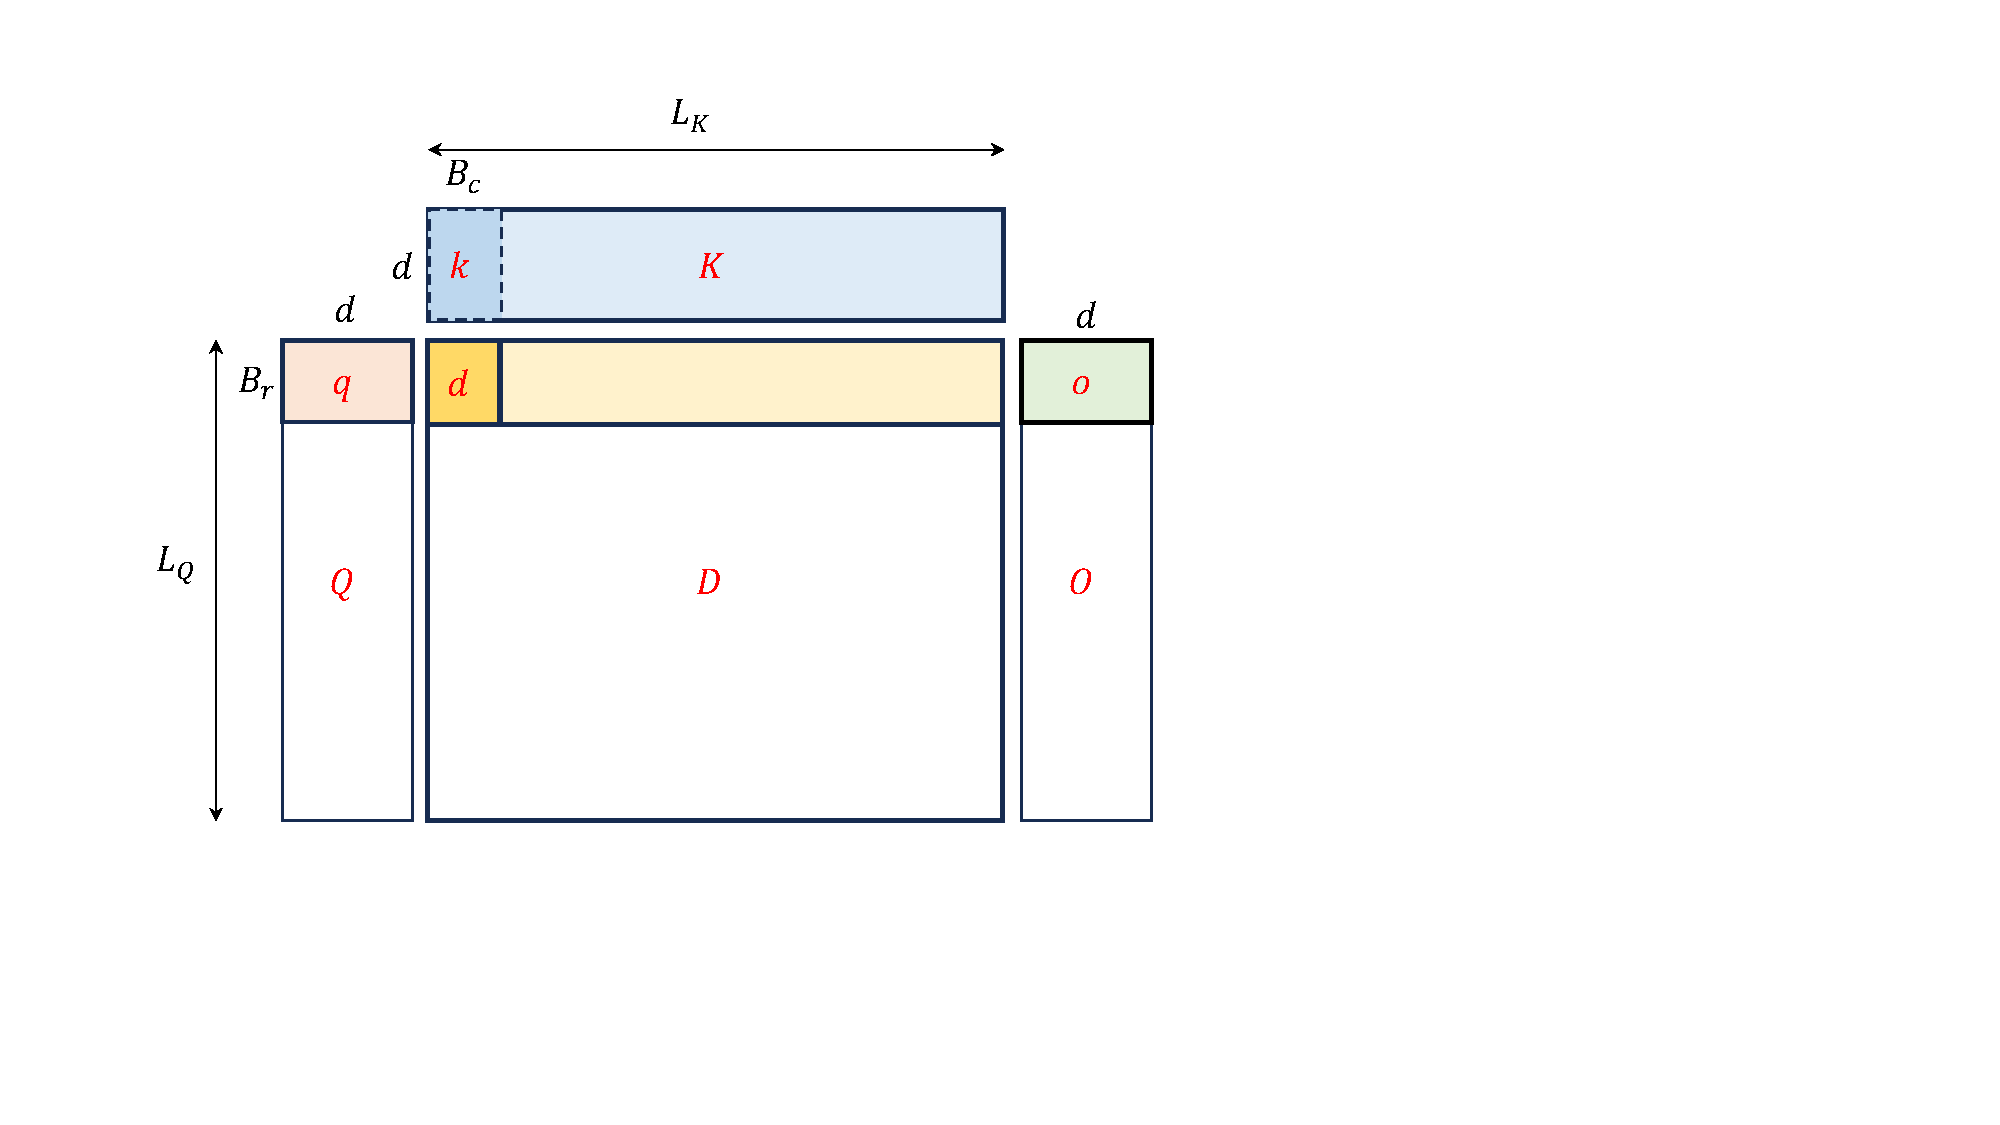
\includegraphics[width=6cm]{figures/attention_offset-a.pdf}
  }\vspace{-1mm}
  \subfigure[{Data accessed by one iteration inside the kernel.}]{
      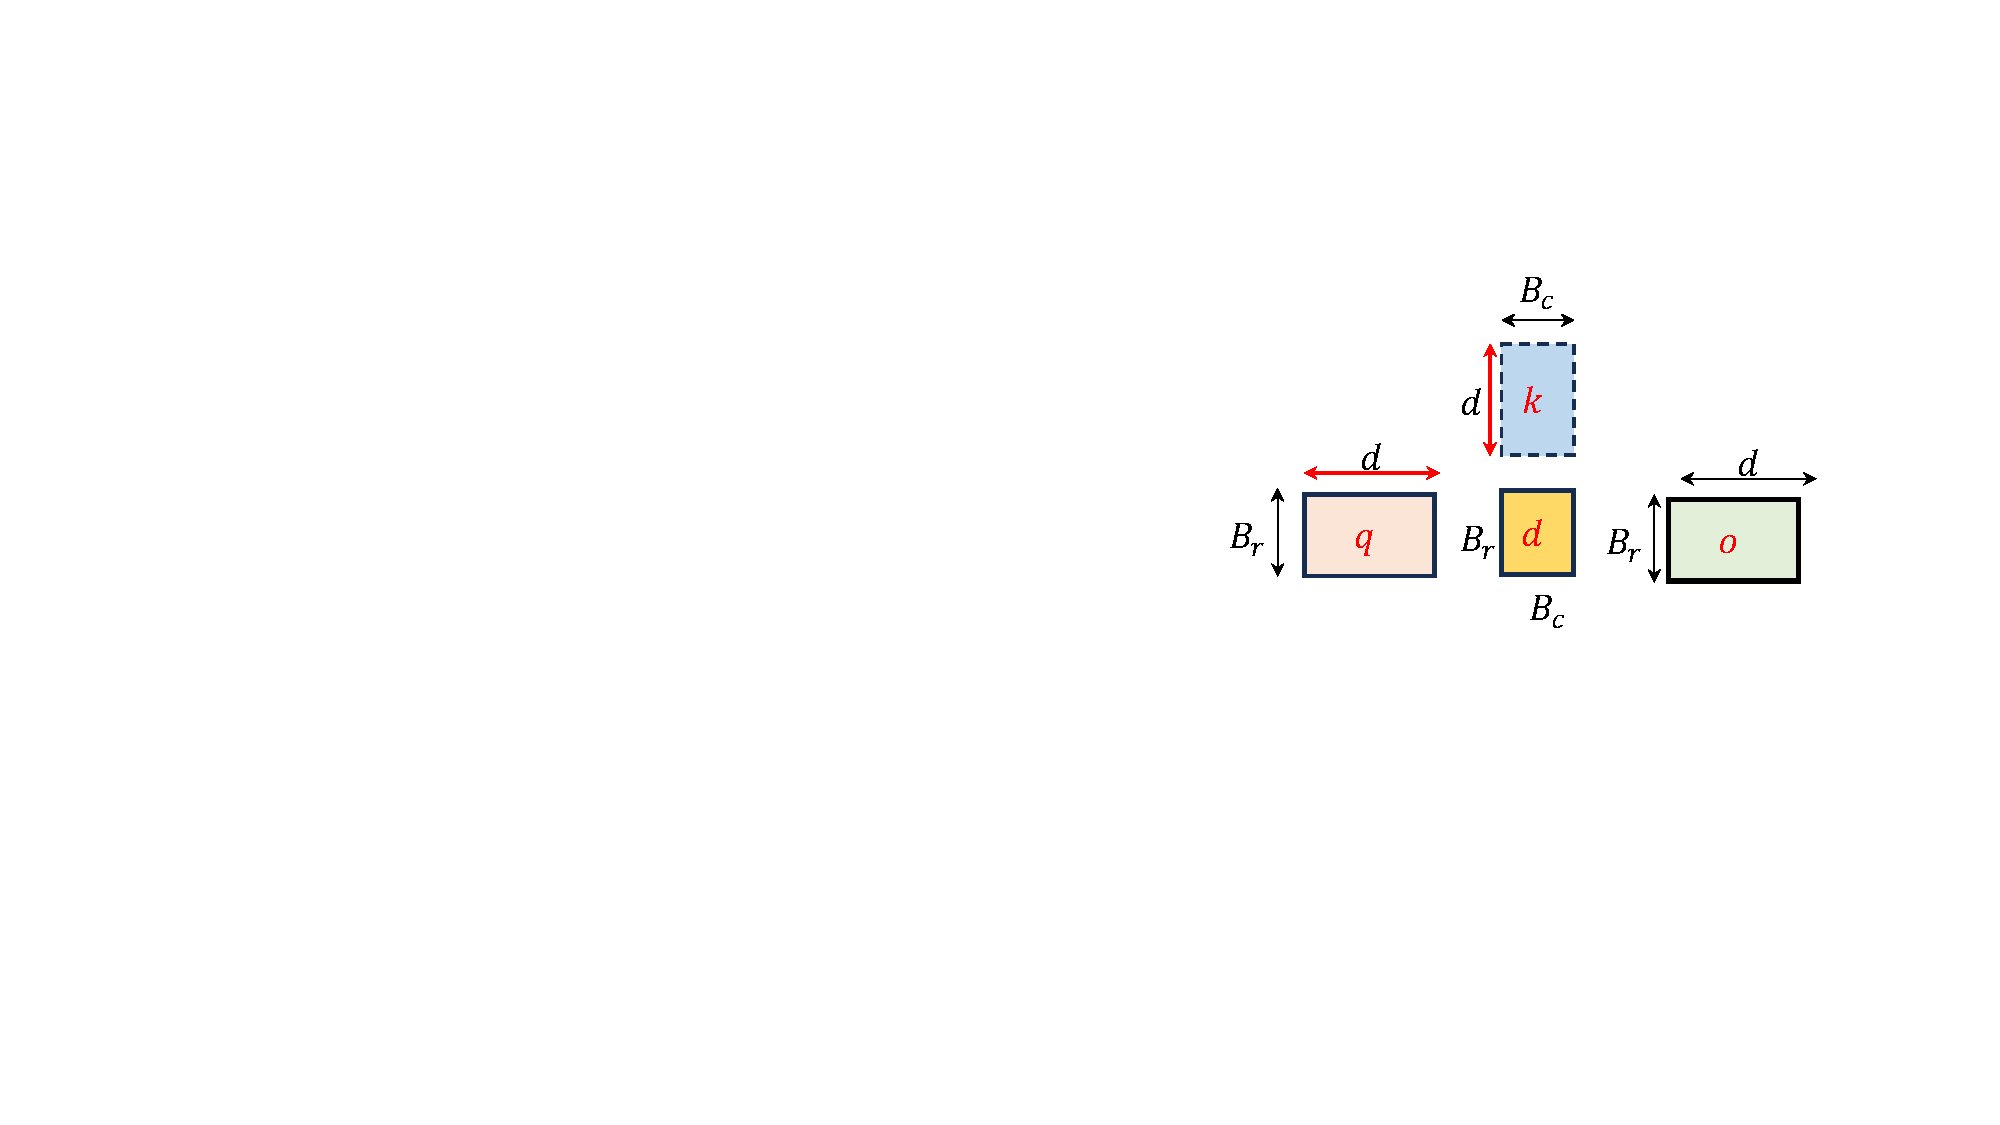
\includegraphics[width=5cm]{figures/attention_offset-b.pdf}
  }\vspace{-1mm}
\end{figure}
\vspace{-0.1cm}

\lstset{
  frame=lrtb,
  backgroundcolor=\color{aliceblue},
  numbers=left,
  numbersep=1em,
  xleftmargin=1em,
  breaklines=true,
  linewidth=\linewidth
}
\begin{lstlisting}[language=code_example2, caption={}]
// ------   Step 1: each CTA gets its input data.   ------
(:$\text{Q\_offset} = \textcolor{blue}{\text{blockIdx.x}} * d * B_r$:)  // offset
(:$\text{D\_offset} = \textcolor{blue}{\text{blockIdx.x}} / N * B_r * L_K$:)  // offset
(:$\text{K\_offset} = \textcolor{blue}{\text{blockIdx.x}} / T_r * d * L_K$:)  // offset

(:$Q = \mathbf{Qs}[\text{Q\_offset}]$:)  // move the pointer
(:$O = \mathbf{Os}[\text{Q\_offset}]$:)  // move the pointer

(:$K = \mathbf{Ks}[\text{K\_offset}]$:) // move the pointer
(:$V = \mathbf{Vs}[\text{K\_offset}]$:) // move the pointer
(:$D = \mathbf{Ds}[\text{D\_offset}]$:) // move the pointer
for(int i = 0; i < (:$T_c$:); ++i) {
  (:\text{k\_offset} = $i* B_c * d$:) // offset
  (:$k = K[\text{k\_offset}]$:)  // move the pointer

  (:\text{d\_offset} = $i * B_r * B_c$:) // offset
  (:$d = D[\text{d\_offset}]$:)  // move the pointer



  // ------   thread in the CTA offset gets its input  ------
}
\end{lstlisting}

\textbf{Notations}:

\begin{itemize}
  \item $N$ stands for batch size, $H$ stands for head number, $L_Q$, $L_K$ and $L_V$ stands for $Q$, $K$, $V$ lengths respectively.
  \item $\mathbf{Qs}$,  $\mathbf{Ks}$,  $\mathbf{Vs}$ stands for the whole input matrix, that has a shape of: $[N*H*L_Q, d]$, $[N*H*L_K,d]$, $[N*H*L_Q, d]$ respectively.
  \item $T_r = \frac{L_Q}{B_r}$: how many blocks along the row dimension.
  \item $T_c = \frac{L_K}{B_c}$: how many blocks along the column dimension.
  \item $Q$,$K$,$V$ stands for inputs to a CTA.
  \item $q$,$k$,$v$ stands for a tile.
\end{itemize}


A single thread block (CTA) reads an \colorbox{NavajoWhite}{orange block} of $Q$; A \colorbox{LightSkyBlue1}{blue block} of $K$ and $V$(\textcolor{byzantium}{$K$ and $V$ are repeatedly load from global memory $T_r$ times}).
Inside a CTA, a sequential \textit{for} loop iterates over \colorbox{LightSkyBlue3}{dark blue blocks} of $K$ and $V$.
\colorbox{DarkSeaGreen}{green block} of $V$.

\textbf{Launch configuration}: $L_Q/B_r * H * N$ blocks are required.

Every $T_r$ blocks repeatedly load $K$ and $V$.

\noindent \textcolor{blue}{\textbf{Input:}} $\mathbf{Qs}, \mathbf{Ks}, \mathbf{Vs}$

